\documentclass[conference]{IEEEtran}
\usepackage{graphicx}
\graphicspath{{fig/}}
\usepackage{amsmath, amssymb}
\usepackage{algorithm, algpseudocode}
\newtheorem{theorem}{Theorem}
\newtheorem{lemma}{Lemma}[theorem]
\newtheorem{definition}{Definition}
\usepackage{hyperref}

\title{AcBF: A Revokable Blockchain-based Identity Management Enabling Low-Latency Authentication}
\author{Jianan Hong, Jia Cheng, Yuqing Li, Jiayue Zhou, and Yue Wu}
\begin{document}
\maketitle

\begin{abstract}
	Blockchain-based identity has brings great evolution due to its decentralized deployment, transparent and tamper-free ledger. Specification groups of B5G/6G are exploring approaches to integrate the technology to future network systems, e.g., Internet of Things, vehicular network, industrial communications. Note that devices in these systems are storage constrained with instable channels, thus requires lightweight node deployment. The security problem comes: revoked identity can forge a legitimate authentication, since the lightweight verifier does not maintain the revocation transactions. 
	This paper hence proposes AcBF, a novel revokable identity management scheme. Especially, it enables extremely low authentication latency by allowing the lightweight node to query certificate's status locally. To realize this feature trustly, we first design a revocation transaction based on accumulator-assisted bloom filter to minimize the storage of certificate status structure. Secondly, we further construct the blockchain protocol, with which, no revocation event will slip on any lightweight ledger, even in an insecure or instable communication environment.  
	In addition, different with other no-CRL revocation mechanism, AcBF brings very small effect to valid user to execute the revocation, with quite a small probability.
	Security and performance analysis
	shows that AcBF has sufficient security and advantageous efficiency on both lightweight verifiers and identity owners, thus suits identity management systems with low-latency constraints.
\end{abstract}
\begin{IEEEkeywords}
    Blockchain identity, revocation-aware authentication, lightweight node, low latency
\end{IEEEkeywords}

\section{Introduction}
Blockchain is an attractive technology for distributed identity management \cite{9075663} due to its security features, such as append-only and non-tempering storage, decentralized consensus, and reliable trust establishment. Compared with traditional identity system, such as PKI (public key infrastructure), the character of blockchain-based method suits better in current and future network systems, due to its ability to faithfully organize the trust for large amount of entities \cite{certchain2018,yang2018blockchain}, particularly the trust relationship between CAs (certificate authorities). 
Therefore, the idea of blockchain-based identity can develop security for various network scenarios, including Internet of Thing (IoT) \cite{zhangBPAFBlockchainEnabledReliable2022a}, Internet of Vehicles (IoV)  \cite{8010820,singh2018branch}, etc., where decentralized trust is critically required. 

Despite the decentralized trust organization introduced by blockchain, it also brings in many practical problems due to its certificate status query method. For blockchain-based identity, a certificate's status (e.g., registered, illegal, or revoked) should be queried from the ledger of blockchain, which is maintained by multiple blockchain nodes. That is the cause of problems or security threats for communication resource-constrained scenarios. Firstly, the transaction query requires several round trip time (RTT) between IoT devices (or vehicle) and at least one blockchain node, which costs unbearable delay for latency-strict cases, e.g., safety notification message of IoV; what is worse, the highly dynamic topology of these network system makes the routing of query response complex. Secondly, it is dangerous to  query certificate's status from only one node, which leads to the security bottleneck problem; and it makes the first problem even worse to refer to more blockchain nodes. A worse threat is that some network attack will isolate the device from legal blockchain nodes at the very time when the device needs to check a certificate. 
It is intuitive but infeasible to let every device keep up with the whole ledger of blockchain, since the distributed devices are lightweight nodes for resources, especially storage. 

This paper proposes a blockchain-based identity management scheme by deploying lightweight blockchain nodes. Rather than stores the whole data, a lightweight node only stores the block header information of each block, thus help the storage-constrained devices to check transaction status locally, with the method of \textit{simplified payment verification} (SPV). As a result, the validity check of identity is completed with extremely low latency, regardless of the communication quality or network attack. 

The property of lightweight node has attracted many researchers to deploy blockchain in IoT, industrial environments, etc.. However, we should take more issues into account, before utilizing it to manage users' and devices' identities. The core problem is revocation! Let us take the following instance: a user's $U$ identity is registered in block $i$, and is later revoked in block $j$. If $U$ wants to authenticate its identity to a lightweight node, it can easily succeed in this forge: as $U$'s certificate still has a valid SPV method for block $i$, and the lightweight node is not informed of the revocation based on the stored block headers, unless $U$ consciously hands it up. Although some blockchain-based identity management schemes have proposed well designed revocation method \cite{luoScalaCertScalabilityOrientedPKI2022a,  wang2020blockchain,jiaRedactableBlockchainDecentralized2022,chenCertchainPublicEfficient2018a}, they no longer work in our system, as they require the verifier to master the whole blockchain data. 

The work presented in this paper aims at proposing a trusted blockchain-based identity management scheme, whose authentication method well resists the revoked users' forging. The proposed work uses a short Bloom Filter to record the revoked certificates; and additionally leverages a pairing-based accumulator to achieve a precise certificate validity check, even with quite small storage. Different from related work, in order to tolerate the case when the forger controls the downlink channel (to obtain block header), we construst our new blockchain scheme (AcBF). In AcBF, with our designed revocation transaction and small-volume header structure, the lightweight verifier can be aware of the revocation events even with the received header, thus achieves local query to improve the efficiency and reliability. 

In summary, this paper makes the following contributions:
\begin{enumerate}
	\item We propose a lightweight on-chain certificate management, where the authentication phase costs negligible overhead to validate the status of the certificate. Specially, the CRL is composed by designed accumulator-assisted bloom filter, thus the filter length can be drastically shortened without the problem of false detection. 
	\item To the best of our knowledge, we are the first to enable low-latency and trusted authentication by constructing a blockchain scheme (AcBF), which makes the lightweight node be aware of revocation event according to block header. As a result, the identity status can be queried locally by the resource-constrained verifiers.
	\item We implement AcBF in our tested environment, and evaluate its performance in terms of computation and storage overhead in various procedures. Results show that AcBF informs every revocation to lightweight node, even in untrust network environment, and the overhead is extremely small on both certificate owners and verifiers, thus quite suit scenarios like IoT and IoV.
\end{enumerate}

The rest of this paper is organized as follows. We will
introduce necessary preliminaries in Section \ref{sec:preliminary}, and in Section \ref{sec:model} we present the system model, followed with the security requirements of AcBF. Detailed Construction is presented in Section \ref{sec:construction}. Then formal security proof and experimental result analysis are shown in Section \ref{sec:security} and \ref{sec:efficiency}, respectively. Section \ref{section:related} briefly discusses the related work. Finally, in Section \ref{sec:conclusion}, we conclude this paper. 


\section{Preliminaries}\label{sec:preliminary}

\subsection{Bilinear Pairing}
Let $\mathbb{G}_1$, $\mathbb{G}_2$ and $\mathbb{G}_T$ be 3 groups of prime order $p$. A pairing map $e:\mathbb{G}_1\times \mathbb{G}_2\rightarrow\mathbb{G}_T$ satisfies:
\begin{itemize}
	\item \textit{Bilinearity:} for all $(x,y, g_1, g_2) \in \mathbb{Z}_p^2\times \mathbb{G}_1\times \mathbb{G}_2$, $e(g_1^x, g_2^y) = e(g_1, g_2)^{xy}$;
	\item \textit{Non-degeneracy:} if $g_1, g_2$ are generators of $\mathbb{G}_1$ and $\mathbb{G}_2$, respectively, $e(g_1, g_2)$ generates $\mathbb{G}_T$;
	\item \textit{Efficiency:} It is efficient to compute $e(u,v)$ for all $(u, v) \in \mathbb{G}_1\times \mathbb{G}_2$.
\end{itemize}

According to the relationship of $\mathbb{G}_1$ and $\mathbb{G}_2$, there are three types of pairings \cite{GALBRAITH20083113}. 
In Type 1, $\mathbb{G}_1 = \mathbb{G}_2$; In Type 2, $\mathbb{G}_1 \neq \mathbb{G}_2$, but there is a unidirectional homomorphism $\phi:\mathbb{G}_2 \rightarrow \mathbb{G}_1$; An in Type 3, no PPT homomorphism algorithm exists between the two groups.
Overall speaking, Type 3 pairings are more secure and efficient to map, which is used in this paper.

Consider the $q$-Strong Diffie-Hellman Problem ($q$-SDH) as follows: given a tuple $(g_1, g_2, g_2^{\gamma}, g_2^{(\gamma^2)}, \dots, g_2^{(\gamma^q)})$ as input, where $g_1\in\mathbb{G}_1$, $g_2\in\mathbb{G}_2$, and $\gamma\in \mathbb{Z}_p$, outputs a pair $(g_1^{1/(\gamma + x)}, x)$ where $x \in \mathbb{Z}_p$. We say that an algorithm $\mathcal{A}$ has advantage $\epsilon$ in solving $q$-SDH if it has probability $\epsilon$ to return the valid pair.

\begin{definition}[$q$-SDH Assumption]
	No PPT algorithm $\mathcal{A}$ can has a non-negligible advantage $\epsilon$ for $q$-SDH problem.
\end{definition}


\subsection{Bloom Filter}\label{section:bf}
Bloom filter (or BF for short) is a space-efficient data structure to record a set, in order to support membership queries \cite{Bloom1970, broder2004network}.
BF is an array of $m$ boolean bits, whose initial status is all zeros (denoted as $0^m$). Another parameter $k$ is the number of independent hashes, each of which maps a member to a random bit of BF. The follows describe the functions of BF, which are to be used in the later context.

\begin{itemize}
    \item $BF.Add(x)$: To add an element $x$ to BF, it respectively hashes $x$ with the $k$ hashes of BF, and sets each of the mapped bit to 1.
	\item $BF.Check(x)$: To query if $x$ has been added, it uses the $k$ hashes to map $x$ to a set of bits. If any of them is 0, it returns False; otherwise, it returns True. 
\end{itemize}

Especially, the $BF.Check()$ gives a False result with no doubt; whereas the True result has the potential to happen when the tested element has not been added, which means a false positive situation. 

\subsection{Merkle Tree and Simplified Payment Verification (SPV)}
\label{section:merkle}
Merkle hash tree \cite{daiSBLWTSecureBlockchain2018} is essentially a binary tree where the leaf node is labeled a hash of a data block, and the non-leaf node is labeled with the hash of its child nodes. Such structure allows efficient verification of any large data. As shown in Fig. \ref{fig:mht}, $cert_A$ is labelled with the 2nd leaf of MHT, whose path is ``01'' (0 for left child and 1 for the right).

Simplified payment Verification (SPV) is a method to check if one data block is in a MHT, when the verifier only knows the root node. To realize the verification, SPV requires the prover side to offer necessary auxiliary information to the verifier, which means the values of \textbf{all sibling nodes from the hash of proved data block to the root}.
Return to Fig. \ref{fig:mht}, the auxiliary information of $cert_A$ is as: $AUX_A = (h_{00}, h_{1})$. Since each one obtaining the auxiliary as well as  $R$ can check if:
\begin{align}\label{eq:aux}
	R \overset{?}{=} h(h(h_{00}, h(cert_A)), h_1)
\end{align}
%where $h()$ is any selected secure hash function.

\begin{figure}[t]
	\centering
	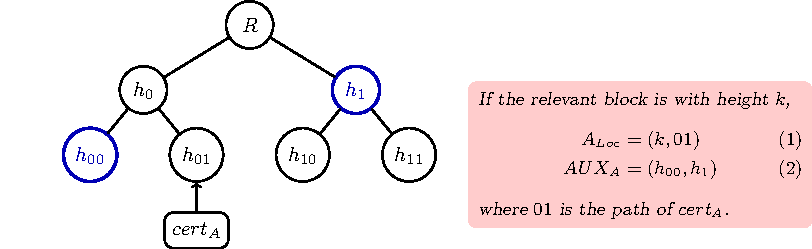
\includegraphics[width=9cm]{mht}
	\caption{Architecture}\label{fig:mht}
\end{figure}

\section{System and Security Model} \label{sec:model}
As shown in Fig. \ref{architecture}, the proposed scheme works in a communication system with the following 3 kinds of entities: multiple CAs, lightweight nodes and a set of blockchain full nodes. The follows describe each of the entities. 

\begin{itemize}
	\item The CAs play the similar role as those in traditional PKI systems, which are responsible for issuing and revoking certificates for other entities. 
\end{itemize}


\section{Construction}\label{sec:construction}
\subsection{Revocation-Aware Block Format}
The block structure in this paper is basically similar to that of Bitcoin, except for the consideration of lightweight node awareness. Firstly, the storage cost of block header should be as short as possible with efficient query and sacrificing no security feature; Secondly, the block header alone can prompt every certificate revocation clearly. 

Taking into account the two issues, we redesign the 1) fields of block header, and 2) the tree structure of transactions. The header is a fixed length data, such that an unstructured storage can support fast addressing based on block height. The necessary fields are depicted in Table \ref{table:format}. Especially, as our later implementation uses 224-bit hash function and curves, the presented sizes of Previous hash and MHT (hash of merkle hash tree) are 28 bytes. The Flag filed is a main difference for the second consideration: it is a boolean variable to notify whether revocation events occur in this round.

The consensus filed depends on the used consensus method, e.g., it is a nonce for puzzle-like consensus method like PoW, or a digital signature for permission-based consensus.


\begin{table}[h] 
	\caption{Block Header Format}\label{table:format}
	\centering
	\begin{tabular}{c|c|l}
		\hline
		Field & Size & Description \\
		\hline
		Height & 4 bytes & An incremental integer to identify this block \\
		Previous Hash & 28 bytes & A hash of previous block \\
		Flag & 1 bit & Indication of revocation \\
		MHT & 28 bytes & Hash of all transactions in this block \\
		Consensus & \textit{variable} & Some method proving the validity of block\\
		\hline
	\end{tabular}
\end{table}

All registered certificates (regarded as transactions) are structured in merkle hash tree as Section \ref{section:mht}, whose hash of root node is represented as $R_c$. There is also a slight difference for revocation awareness: if there is no revocation, $R_c$ is just the value of MHT; otherwise, MHT is assigned the hash of $R_a$ and the signature of revocation transaction in this block (denoted as $R_x$). For certificates registered in this block, their SPV data includes $R_x$ in such case.


\subsection{System Procedures}

\subsubsection{Initialization}
The rCA initiates the system by generating a bilinear tuple $PP=\{p, \mathbb{G}_1, \mathbb{G}_2, \mathbb{G}_T, g_1, g_2, e\}$ and a hash function $H:\{0, 1\}^* \rightarrow \mathbb{Z}_p$. It selects its master secret key $\gamma\in \mathbb{Z}_p$, accumulator value $\Delta\in_R \mathbb{G}_1$, 
and parameters of Bloom filter $(m, k)$ as Section \ref{section:bf}, based on the expected system scale as Section \ref{section:parameter}. It further generates an empty revocation list $\mathbb{R}_x$. The system parameters are published as 
$$ \bigl\{ PP, \Delta, Y = g_2^\gamma, (m, k) \bigr\}$$

Blockchain full nodes are gathered by generating a genesis block $B_0$, whose header's format follows Table \ref{table:format}, with all-zeros fields, except the consensus. 

The iCAs are registered in the blockchain as Section \ref{section:register}. As a distributed system, iCA's certificates should be registered in self-sovereign manner, while our AcBF also supports rCA's issuing, by using key pair $(\gamma, Y)$ with BLS signature \cite{boneh2004short}. Note that, iCA's certificate status is queried like other entities', hence the later content will not specifically describe the iCA's status check in authentication phase. 

\subsubsection{Certificate Register}\label{section:register}
From an arbitrary trusted iCA, each entity $U_i$ applies this phase to register an on-chain certificate $cert_i$. The certificate in AcBF is basically similar to that in X.509, except that AcBF does not need the globally unique sequence number. Instead, AcBF uses its unique locate $i_{Loc} = (i_h, i_p)$ in blockchain to identify the certificate, where $i_h$ is denoted as the height of registered block, and $i_p$ is its path in MHT. 

We should mention that $U_i$ securely stores a secret key $sk_i$, whose relevant public key $pk_i$ is included in $cert_i$. The $U_i$ should wait for this certificate to be gathered with other transactions (including registration and revocation transactions) 

\subsubsection{Revocation}

\begin{algorithm}
\renewcommand{\algorithmicensure}{\textbf{Output:}}
	\caption{Revocation Procedure of rCA}\label{alg:cap}
	\begin{algorithmic}[1]
		\Require $\mathbb{R}$, $\mathbb{R}_x$, $BF$ and $\Delta$ %\Comment{Set of user indexes to be revoked}
		\Ensure Revocation Transaction ($rx$)
		\State $L\gets \emptyset$
		%\State $\Delta_T \gets \Delta$
		\State $BF_{tmp} \gets 0^m$ \Comment{Empty bloom filter}
		\ForAll{$x \in \mathbb{R}$}
		\If{$BF.Check(x)$} \Comment{as Section \ref{section:bf}}
		\State $\Delta \gets Del(\Delta, x)$ 
		\State append $(x, \Delta)$ to L
		\Else
		\State $BF_{tmp}.Add(x)$ \Comment{as Section \ref{section:bf}}
		\EndIf
		\EndFor
		\State $BF \gets BF \lor BF_{tmp}$
		\State $\mathbb{R}_x \gets \mathbb{R}_x \bigcup \mathbb{R} $
		\State $rx \gets (L, \mathbb{R})$
	\end{algorithmic}
\end{algorithm}



\subsubsection{Authentication}


\subsubsection{Block Generate and Broadcast}
The consensus nodes collect certificate register and revocation transactions 
\subsection{Parameter Determine for Bloom Filter} \label{section:parameter}

The length of Bloom Filter in this paper can be dramatically decreased compared with other schemes for certificate revocation. This section gives a theoretical derivation for the relevant parameter.

Let $n, \delta$ be the possible maximal number of registered and revoked users, respectively. The remaining factor is system effect of user revocation: when revocation is executed in one consensus round, the expected affected users should be limited to $\theta$, which can be measured as the member amount of Accumulator $\Delta$. The measurement is feasible as:
\begin{itemize}
    \item Larger member amount in $\Delta$ causes larger probability that a user to be revoked has already in $\Delta$ and more other members to update their auxiliary information as \eqref{xxx}.
    \item The probability that innocent users applies for accumulator member affects the increase rate of $\theta$. Thus, $\theta$ also implies the effect when revocation is executed just in bloom filter.
\end{itemize}

Assume $m$ is the calculated hash length with $k$ hash functions in the Bloom filter. With $\delta$ users already be revoked, the probability can be measured as follows, that an legal user is erroneously claimed as a revoked one: 
\begin{align} 
    \Pr(1) \simeq (1 - e^{-k\delta/m})^k 
 \end{align}

The parameter $k$ can be individually optimized to minimize $\Pr(1)$ as $ k = \frac{m}{\delta}\ln 2$. Then, for $n$ valid users, the expected affected amount (limited to $\theta$) is 
\begin{align}\label{eq:bloomfilter}
    \theta = n \cdot (1 - e^{-k\delta/m})^{k} = 0.5^{\frac{m}{\delta}\ln 2}\cdot n
\end{align}
From \eqref{eq:bloomfilter}, the parameters of Bloom filter can be determined as 
\begin{align}
m = & \frac{\ln \frac{n}{\theta} \cdot \delta}{(\ln 2)^2} \simeq 2.08\delta \cdot\ln \frac{n}{\theta}\\
k = & \lfloor \ln \frac{n}{\theta} / \ln 2 \rceil \simeq \lfloor 1.44 \ln \frac{n}{\theta} \rceil
\end{align}

%\subsection{Compatibility on Other Blockchains}
%We recommend to implement AcBF with designed block header structure as Table \ref{table:format}, but it is also compatible with traditional blockchain implementations. The main challenge is that Flags

\section{Security Analysis of AcBF}\label{sec:security}
\begin{theorem}\label{theo:security}
	The AcBF identity management achieves sound and revocation-detectable user authentication for the lightweight-node verifier.
\end{theorem}

\begin{IEEEproof}
    A user without a registered certificate in public ledger (even without a revoked identity) will not forge an authentication due to the traditional certificate technique with trust SPV method. Thus, this proof mainly focuses on the revoked user. Formally, this theorem holds if a revoked user $\mathcal{A}$ wins the following challenges with negligible advantage.
    \begin{enumerate}
        \item With the knowledge of accumulator value $\Delta$, as well as any pair of other user's accumulator pair from authentication message \ref{section:authentication}, $\mathcal{A}$ tries to forge its auxiliary value.
        \item When $\mathcal{A}$ goes through a revocation based on member delete in $\Delta$, it tries to forge a new auxiliary value for the updated $\Delta$.
        \item When $\mathcal{A}$ is revoked in block $j$, it tries to hide the revocation fact during the broadcast of block header.
    \end{enumerate}

    The first 2 challenges require a secure cryptographic accumulator, and a strong blockchain protocol is in need for the last challenge. Hence, the demonstration of Theorem \ref{theo:security} can be derived from the following 2 lemmas.
\end{IEEEproof}
\begin{lemma}
    accumulator
\end{lemma}

\begin{lemma}
    If the consensus protocol of the used blockchain is safe, the lightweight node is aware of every revocation when its ledger has been updated to relevant status.
\end{lemma}

\begin{IEEEproof}
When a certificate is successfully revoked in a block (e.g., of height $i$), the Flag field of its header should be \textit{True}. As long as the consensus protocol has a strong safety property, the lightweight node will not accept the $i$-th block header with Flag field \textit{False}. 
\end{IEEEproof}

\section{Performance Evaluation} \label{sec:efficiency}

Compared with entire bloom filter with distinct parameters.

\section{Related Works}\label{section:related}

\section{Conclusion}\label{sec:conclusion}

\bibliographystyle{IEEEtran}
\bibliography{id}
\end{document}